\documentclass[12pt]{amsart}
\setlength{\parskip}{.1in}
\setlength{\parindent}{0cm}
%myalterations
\usepackage{amssymb}
\usepackage{amsmath}
\usepackage[usenames,dvipsnames,svgnames,table]{xcolor}
\usepackage[colorlinks=true,urlcolor=blue,pdfborder={0 0 .5}pdfnewwindow=true]{hyperref}
\usepackage{enumitem}
%\usepackage{amsthm}
\usepackage{graphicx}
\usepackage{float}
\usepackage{verbatim}
\usepackage{tabularx}
%\usepackage{arydshln,leftidx,mathtools}
\usepackage{bm}
\usepackage{tikz}
\usepackage{tikz-cd}
\usepackage{hyperref}
\usepackage{bm}
\usepackage{wasysym}
%\setlength{\dashlinedash}{.4pt}
%\setlength{\dashlinegap}{.8pt}
%\usepackage{amsthm}
\usepackage{verbatim}
%\usepackage{commath}
%My commands
%environment abbreviations
\newcommand{\benu}{\begin{enumerate}}
\newcommand{\eenu}{\end{enumerate}}
\newcommand{\bed}{\begin{description}}
\newcommand{\ed}{\end{description}}
\theoremstyle{definition}
\newtheorem{theorem}{Theorem}
\newtheorem{notation}[theorem]{Notation}
\newtheorem{exercise}[theorem]{Exercise}
\newcommand{\bex}{\begin{exercise}}
\newcommand{\ex}{\end{exercise}}
\newtheorem{definition}[theorem]{Definition}
\newcommand{\bdf}{\begin{definition}}
\newcommand{\edf}{\end{definition}}

%symbol definitions
\newcommand{\un}[1]{\underline{#1}}
\newcommand{\mbZ}{\mathbb{Z}}
\newcommand{\mbR}{\mathbb{R}}
\newcommand{\mbN}{\mathbb{N}}
\newcommand{\mbQ}{\mathbb{Q}}
\newcommand{\mbC}{\mathbb{C}}
\newcommand{\mbF}{\mathbb{F}}
\newcommand{\mcS}{\mathcal{S}}
\newcommand{\mcP}{\mathcal{P}}
\newcommand{\hra}{\hookrightarrow}
\newcommand{\tra}{\twoheadrightarrow}
\newcommand{\lra}{\leftrightarrow}
\newcommand{\ep}{\epsilon}
\newcommand{\Ra}{\Rightarrow}
\newcommand{\mb}[1]{\mathbb{#1}}
\newcommand{\mc}[1]{\mathcal{#1}}
\newcommand{\bfs}[1]{{\bfseries #1}}
\newcommand{\bs}[1]{\boldsymbol{#1}}
%Operator definitions
\DeclareMathOperator{\Irr}{Irr}
\DeclareMathOperator{\triv}{triv}
\DeclareMathOperator{\cyc}{cyc}
\DeclareMathOperator{\lcm}{lcm}
\DeclareMathOperator{\expo}{x}
\DeclareMathOperator{\ord}{o}
\DeclareMathOperator{\imm}{im}
\DeclareMathOperator{\sgn}{sgn}
\DeclareMathOperator{\Sym}{Sym}
\DeclareMathOperator{\alt}{alt}
\DeclareMathOperator{\irr}{irr}
\DeclareMathOperator{\eqt}{Equiv}
\DeclareMathOperator{\pat}{Part}
%\DeclareMathOperator{\sgn}{sgn}
%\DeclareMathOperator{\Aut}{Aut}
\DeclareMathOperator{\Gl}{Gl}
\DeclareMathOperator{\M}{M}
\DeclareMathOperator{\Id}{Id}
\DeclareMathOperator{\fixx}{Fix}
\DeclareMathOperator{\suppp}{Supp}
\DeclareMathOperator{\gl}{Gl}
\DeclareMathOperator{\id}{Id}
\DeclareMathOperator{\Aut}{Aut}
\DeclareMathOperator{\Inn}{Inn}
\DeclareMathOperator{\orb}{orb}
\DeclareMathOperator{\ii}{I}
\DeclareMathOperator{\im}{im}
\DeclareMathOperator{\Fix}{Fix}
\DeclareMathOperator{\Co}{Co}
\DeclareMathOperator{\md}{md}
\DeclareMathOperator{\qt}{qt}
\DeclareMathOperator{\ExtendedGCD}{ExtendedGCD}
\DeclareMathOperator{\Mod}{Mod}
\DeclareMathOperator{\GCD}{GCD}
\newcommand{\nms}{\negmedspace}
\newcommand{\nts}{\negthinspace}

\newcommand{\itep}{\item {\bfseries Problem}\ }
\newcommand{\gen}[1]{\langle \nts#1 \nts\rangle}
\newcommand{\quot}[2]{#1/ #2}
\newcommand{\order}[1]{\left|<\nts #1 \nts s>\right|}

%These next two commands are for making answers. 
\newcommand{\beans}{\begin{description} \item[{ \bfseries \textcolor{red}{Answer}}]\ }
\newcommand{\eans }{\end{description}}
%\newcommand{\begin{comment}ex}{{ \bfseries \textcolor{red}{Answer}}}

%To turn the answer into problem sets use replace to replace \begin{comment} with \begin{comment} and \\end{comment}  by \end{comment}.
\newcommand{\lieb}[3][{{}}]{\frac{d^#1 #2}{d\,#3^#1}}

\title{\textbf{Math 521 - Problem Set 1}}
\author{Guy Matz}
\date{\today}

\begin{document} 

\maketitle
\newpage % Q1

\begin{enumerate}[series=p]
\itep 1
\\
Prove that for all set $A, B, C$ the formula
$$A \cup (B \cap C) = (A \cup B) \cap (A \cup C)$$
is true.
\\
$\Rightarrow$ We want to show that $A \cup (B \cap C) \subseteq (A \cup B) \cap (A \cup C)$.  That is, an arbitrary element, $x \in A \cup (B \cap C)$ is also in $(A \cup B) \cap (A \cup C)$.  Let $x \in A \cup(B \cap C)$.  Then either $x \in A$ or $x$ is in both $B$ and $C$.  So $x \in A$ or ($x \in B$ and $x \in C$).  Then we have ($x \in A$ or $x \in B$) and ($x \in A$ or $x \in C$), and therefore $x \in (A \cup B) \cap (A \cup C)$
\\\\
$\Leftarrow$ We want to show that $(A \cup B) \cap (A \cup C) \subseteq A \cup (B \cap C)$.  That is, an arbitrary element, $x \in (A \cup B) \cap (A \cup C)$ is also in $A \cup (B \cap C)$.  Let $x \in (A \cup B) \cap (A \cup C)$.  Then $x$ is in $A$ or $B$ and $x$ is in $A$ or $C$.  So $x$ is in $A$ or $x$ is in both $B$ and $C$, hence $x \in A \cup (B \cap C)$
\newpage % Q2

\itep 2
\benu
\item Prove that $(A^c)^c = A$
\\
$\Rightarrow$ We want to show that $(A^c)^c \subseteq A$\\
Let $x \in (A^c)^c$.  So $x \notin (A^c)$. Hence $x \in A$. 
\\
$\Leftarrow$ We want to show that $A \subseteq (A^c)^c$\\
Let $x \in A$.  So $x \notin (A^c)$. Hence $x \in (A^c)^c$. 
\\
\item Prove deMorgan's Law: $(A \cap B)^c = A^c \cup B^c$ and derive from the law $(A \cup B)^c = A^c \cap B^c$.
\\
$\Rightarrow$ We want to show that $(A \cap B)^c \subseteq A^c \cup B^c$.  Let $x \in (A \cap B)^c$.  Then $x \notin (A \cap B)$, so $x \notin A$ or $x \notin B$.  Hence $x \in A^c$ or $x \in B^c$, i.e. $x \in (A^c \cup B^c)$ 
\\\\
$\Leftarrow$ We want to show that $A^c \cup B^c \subseteq (A \cap B)^c$.  Let $x \in A^c \cup B^c$.  So $x \in A^c$ or $x \in B^c$.  Then $x \notin A$ or $x \notin B$, so $x \notin (A \cap B)$, i.e $x \in (A \cap B)^c$
\\
\\
How to derive $(A \cup B)^c = A^c \cap B^c$?\\
We can say that $A^c \cap B^c = (((A^c) \cap (B^c))^c)^c$, which is in the form of deMorgan's Law.  So, $(((A^c) \cap (B^c))^c)^c = ((A^c)^c \cup (B^c)^c)^c = (A \cup B)^c$
\\
\item Draw Venn diagrams to illustrate the two laws
\begin{figure}[H]
	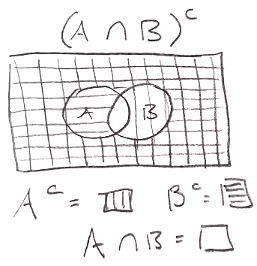
\includegraphics{intersection.png}
	\caption{$(A \cap B)^c = A^c \cup B^c$}
	\label{fig:venn_intersection}
\end{figure}
\begin{figure}
	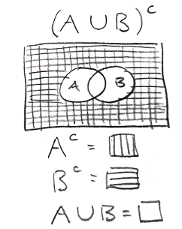
\includegraphics{union.png}
	\caption{$(A \cup B)^c = A^c \cap B^c$}
	\label{fig:venn_union}
\end{figure}

\item Generalize these laws to more than two sets
\benu
\item $(A_1 \cap A_2 \cap \dots \cap A_n)^c = A_1^c \cup A_2^c \cup \dots \cup A_n^c$
\\
\item $(A_1 \cup A_2 \cup \dots \cup A_n)^c = A_1^c \cap A_2^c \cap \dots \cap A_n^c$
\\

\eenu
\eenu 

\newpage
\itep 3\\
Recast the following English sentences in mathematics, using correct mathematical grammar.  Preserve their meaning
\\
\benu
\item 2 is the smallest prime number
\\ Let $p \in \mathcal{P}$ where $\mathcal{P}$ is the set of all primes, $p \geq 2$
\item The area of any bounded plane region is bisected by some line parallel to the x-axis
\\
\\
Let $f$ and $g$ be continuous, integrable functions, and $a < b$.  Then $\exists c \in (a, b)$ such that 
$$\int_{a}^{c}|f(x)-g(x)| dx = \int_{c}^{b} |f(x) - g(x)| dx = \int_{a}^{b} \frac{|f(x) - g(x)|dx}{2}$$
\\
\item All that glitters is not gold
\\Let $X$ be the set of all things that glitter, $Y$ be the set of all things that are gold.  $\exists x \in X$ such that $x \notin Y$
\eenu
\newpage

\itep 9\\
Let $x = A|B, x' = A'|B'$ be cuts in $\mbQ$.  We defined
$$x + x' = (A + A')|\text{ rest of } \mbQ$$
\benu
\item Show that although $B + B'$ is disjoint from $A + A'$, it may happen in degenerate cases that $\mbQ$ is not the union of $A + A'$ and $B + B'$
\\
It may be the case that when two cuts are "open" cuts, i.e. both irrational, then 
\\

\item Infer that the definition of $x + x'$ as $(A + A')|(B + B')$ would be incorrect?
\\
This may not include all of the rationals , so it is not a cut.
\\
\item Why did we not define $x \cdot x' = (A \cdot A')|$rest of $\mbQ$?
\\
If either $x$ or $x'$ is negative, multiplication get "tricky".  See page 14-15
\eenu

\newpage
\itep 10\\
A multiplicative inverse of a non-zero cut $x = A|B$ is a cut $y = C|D$ such that $x \cdot y = 1$
\benu
\item If $x > 0^*$, what are $C$ and $D$?\\
\\
$$C = \{r \in \mbQ : \forall a \in A, a > 0, r < \frac{1}{a}\}$$
$$D = \{r \in \mbQ : \forall b \in B, b > 0, r \geq \frac{1}{b}\}$$
\item If $x < 0^*$, what are they?\\
\\
$$C = \{r \in \mbQ : \forall a \in A, a < 0, r < \frac{1}{a}\}$$
$$D = \{r \in \mbQ : \forall b \in B, b < 0, r \geq \frac{1}{b}\}$$
\\
\item Prove that $x$ uniquely determines $y$
\\
Let $y' \in \mbR$ s.t. $y' \cdot x = 1$.  Then $y = y \cdot 1 = y \cdot (x \cdot y') = (y \cdot x) \cdot y' = y' $
\\
\eenu

\newpage
\itep 12\\
Let $b$ = l.u.b. $S$, where $S$ is a bounded nonempty subset  of $\mbR$.
\benu
\item Given $\epsilon > 0$ show that there exists an $s \in S$ with
$$b - \epsilon \leq s \leq b.$$
\\
Assume towards a contradiction that there is no $s \in S$ such that $b - \epsilon \leq s \leq b$.  Then $b - \epsilon$ is an upper bound of $S$ less than $b$.\hfill \lightning
\\
\\
\item Can $s \in S$ always be found so that $b - \epsilon < s < b$?
\\\\
No.  As a counter-example, choose $S = \{ 1 \}$.  In this case, $b = 1$, however there is no $s$ to satify the inequality above.
\\
\item If $x = A|B$ is a cut in $\mbQ$, show that $x$ = l.u.b $A$.
\\
\benu
\item If $x = A|B$ and $r \in A$, then $r^* < x$
\item If $b = C|D$ is an upper bound of $A^*$, then for all $r \in A$, $r^* \leq b$.  So $\{p \in \mbQ: p < r \} \subseteq C$, and $A = \bigcup\limits_{r \ \in A} \{p \in \mbQ : p < r \} \subseteq C$.  Then, since $x = A|B, x \subseteq b$
\eenu
\eenu

\newpage
\itep 13\\
Prove that $\sqrt{2} \in \mbR$ by showing that $x \cdot x = 2$ where $A|B$ is the cut in $\mbQ$ with $A = \{r = \mbQ: r \leq 0 \text{ or } r^2 < 2\}$.  Hint: Use exercise 12.
\\\\
By 12c we have that $x$ is l.u.b. of $A^*$.  So, for $r^* > 0, (r^*)^2 \leq x^2$.  However, we cannot have $x^2 < 2$ since there are rational numbers as close to 2 as we like.  We also cannot have $x^2 > 2$, for if we say $2 = x^2 - \epsilon$, with $\epsilon > 0$, by 12a there is $r^* \in A^*$ such that $x^2 \geq (r^*)^2 \geq x^2 - \epsilon = 2$.  Hence, $x^2 = 2$


\newpage
\itep 14\\
Given $y \in \mbR, n \in \mbN,$ and $\epsilon > 0$, show that for some $\delta > 0$, if $u \in \mbR$ and $|u-y| < \delta$ then $|u^n - y^n| < \epsilon$.  Hint: Prove the inequality when $n = 1, n = 2$, and then do induction on n using the identity
$$u^n - y^n = (u-y)(u^{n-1} + u^{n-2}y + \dots + y^{n-1})$$
\underline{Base Step}: $n = 2$
\\
If $|u - y| < \delta$, then $|u^2 - y^2| = |(u - y) \cdot (u + y))| < \epsilon$.\\ so $|u -y | < \frac{\epsilon}{|u + y|} = \delta$.  Let's assume that $|u - y | < \frac{1}{2}$, so $-\frac{1}{2}+2y < u+y < \frac{1}{2} + 2y$, and since $\frac{\epsilon}{-\frac{1}{2} + 2y} > \frac{\epsilon}{u + y} > \frac{\epsilon}{\frac{1}{2} + 2y}$, we want to choose $\delta = min(\{\frac{\epsilon}{\frac{1}{2}+2y}, \frac{1}{2}\})$
\\\\
\underline{Induction Hypothesis}:
\\
If $|u - y| < \delta$, then $|u^n - y^n| < \epsilon$  DO I NEED TO SAY SOMETHING HERE ABOUT THE SIZE OF $\epsilon$?
\\\\
\underline{Induction Step}:
\\
\\
If $|u-y| < \delta$, then $|u^{n+1} - y^{n+1}| < \epsilon$\\
$|u^{n+1} - y^{n+1}| = |(u - y)\cdot(u^n + u^{n-1}y + \dots + uy^{n-1} + y^n)|$\\
\\
Now if we assume that $|u - y | < 1$, then $u < y + 1$, and $\frac{\epsilon}{(u^n + u^{n-1}y + \dots + uy^{n-1} + y^n)} > \frac{\epsilon}{(y+1)^n + (y+1)^{n-1}y + \dots + (y+1)y^{n-1} + y^n)}$, we want to choose $\delta = min(\{\frac{\epsilon}{(y+1)^n + (y+1)^{n-1}y + \dots + (y+1)y^{n-1} + y^n)}, 1\})$

\newpage
\itep 15\\
Given $x > 0$ and $n \in \mbN$, prove that there is a unique $y > 0$ such that $y^n = x$.  That is, $y = \sqrt[n]{x}$ exists and is unique.  Hint: Consider
$$y = \text{l.u.b.}\{s \in \mbR : s^n \leq x\}$$

\newpage
\itep 16\\
Prove that real numbers correspond bijectively  to decimal expansions not terminating in an infinite strings of 9's, as follows.  The decimal expansion of $x \in \mbR$ is $N.x_1.x_2\dots$ where $N$ is the largest integer $\leq x, x_1$ is the largest integer $\leq 10(x-N), x_2$ is the largest integer $\leq 100(x-(N+x_1/10))$ and son on.
\\
\benu
\item Show that each $x_k$ is a digit between 0 and 9
\\
Induction on $k: x_k$ is the largest integer less than $10^{k-1}(x-(N  + \frac{x_{k-1}}{10^{k-1}}+ \dots))$
\\\underline{Base Step}:\\
$x_1$ is the largest integer $\leq 10(x - N)$. Since $N$ is the largest integer less than $x$, $0 \leq x - N \leq 1$, and $10(x - N) < 10$.  $x_1$ is the largest integer less than $10(x -N)$ so $0 \leq x_1 \leq 9$
\\
\underline{Induction Hypothesis}:\\
$0 \leq x_k \leq 9$, so $x_k$ is the largest integer less than $10^{k-1}(x-N+\frac{x_{k-1}}{10^{k-1}})$
\\
\underline{Induction Step}:\
$0 \leq x_{k+1} \leq 9$ so $x{k+1}$ is the largest integer $\leq 10^k(x - N + \frac{x_k}{10^k})$

\item Show that for each $k$ there is an $l \geq k$ such that $x_l \neq 9$
\\
Towards a contradiction, assume that there is no $l \geq k$ such that $x_l \neq 9$.  We would then a number 9.99999..., However this number is 1.0\hfill\lightning
\\
\item Conversely, show that for each such expression $N.x_1.x_2\dots$ not terminating in an infinite string of 9's, the set
$$ \{N, N + \frac{x_1}{10}, N + \frac{x_1}{10} + \frac{x_1}{100}\}$$ DO THIS TOMORROW!!
is bounded and its least upper bound is a real number $x$ with decimal expression $N.x_1.x_2\dots$
\\
\item Repeat the exercise with a general base in place of 10.
\eenu

\newpage
\itep *30\\
Suppose that a function $f : [a,b] \Rightarrow \mbR$ is monotone increasing i.e., $x_1 \leq x_2 \Rightarrow f(x_1) \leq f(x_2).$
\benu
\item Prove that $f$ is continuous except at a countable set of points.  [Hint: Show that at each $x \in (a,b), f$ has a right limit $f(x+)$ and a left limit $f(x-)$, which are limits of $f(x+h)$ as $h$ tends to 0 through positive, and negative values respectively.  The jump of $f$ at $x$ is $f(x+) - f(x-)$.  Show that $f$ is continuous at $x$ if and only if it has zero jump at $x$.  At how many points can $f$ have jump $\geq 1$?  At how many points can the jump be between 1/2 and 1?  Between 1/3 and 1/2?]
\\
\item Is the same assertion true for a monotone function defined on all of $\mbR$?
\\
\eenu

\newpage
\itep 36\\
A real number is algebraic if it is a root of a nonconstant polynomial with integer coefficients.
\benu
\item Prove that the set $A$ of algebraic numbers is denumerable.  [Hint: Each polynomial has how many roots?  How many linear polynomials are there?  How many quadratics? . . .]
\\
Each polynomial of order $S$ has $r \leq S$ roots in $\mbR$.  Since there are $\mbN^S$ options for coefficients, there are less than $\mbN^S \cdot S$ elements in the set $A$ of algebraic numbers, so $A$ is denumerable.
\\
\item Repeat the exercise for roots of polynomials whose coefficients belong to some fixed, arbitrary denumerable set $s \in \mbR$
\\
Since the coefficients are fixed, they are denumerable as above.
\\
\item Repeat the exercise for roots of trigonometric polynomials with integer coefficients.
\\
The roots of trigonometric polynomials include the transcendental numbers, which are denumerable as above.
\eenu

\end{enumerate}
\end{document}
